\subsection{Color Bordes}
La finalidad de este filtro es la detección de bordes de la imagen sobre los pixeles lindantes de cada pixel, para eso calcula las diferencia tanto del eje horizontal como del vertical de los 8 pixeles y luego las suma. En este caso se deja un marco de 1 pixel de color blanco alrededor de toda la imagen, por lo que nos ahorramos los problemas de los casos borde.

\subsubsection{Pseudocódigo del ciclo:}
\begin{codesnippet}
\begin{verbatim}
Para i de 1 a height - 2;
    Para j de 1 a width - 2; 
        r=0, g=0, b=0;
        Para ii de i-1 a i+1
            r += abs(src_matrix[ii][j-1].r - src_matrix[ii][j+1].r);
            g += abs(src_matrix[ii][j-1].g - src_matrix[ii][j+1].g);
            b += abs(src_matrix[ii][j-1].b - src_matrix[ii][j+1].b);
        Para jj de j-1 a j+1
            r += abs(src_matrix[i-1][jj].r - src_matrix[i+1][jj].r);
            g += abs(src_matrix[i-1][jj].g - src_matrix[i+1][jj].g);
            b += abs(src_matrix[i-1][jj].b - src_matrix[i+1][jj].b);
        dst_matrix[i][j].r = SATURAR(r);
        dst_matrix[i][j].g = SATURAR(g);
        dst_matrix[i][j].b = SATURAR(b);
\end{verbatim}
\end{codesnippet}

\subsubsection{Implementación del ciclo en ASM}

Dado que alrededor de la imagen va a haber un marco de 1 pixel blanco, se declara una variable para dejar cuatro pixeles en blanco y otro para setear la transparencia en 255 para dos pixeles.
\begin{codesnippet}
\begin{verbatim}   
    blanco: TIMES 4 db 255, 255, 255, 255
    transparencia: TIMES 2 db 0, 0, 0, 255
\end{verbatim}
\end{codesnippet}

En cada ciclo se debe operar con los pixeles lindantes del pixel [i],[j], aprovechando el tamaño de los registros \textbf{XMM} se cargaran en 3 de estos 15 bytes, es decir4 pixeles, un registro para cada fila [i], [i-1] e [i+1] lo que permitirá procesar de a dos pixeles la imagen \textbf{dst}, porque para cada pixel se necesitan tanto los pixeles de la columna y fila anterior como los de las siguientes, al procesar de a dos pixeles se necesita 4 pixeles en lugar de 3 de cada fila. En la figura ~\ref{bordes1}\\
El registro con el que se hace el recorrido de la imagen \textbf{src} en el ciclo apunta al pixel [0][0], haciendo referencia a el pixel [i-1][j-1] en el pseudocódigo, que avanzará 2 pixeles en cada ciclo en mayor parte. En cambio cuando se esté a 4 pixeles del final de la fila, se avanzará 4 pixeles, comenzando el ciclo en una nueva fila. \\ Aprovechando el parámetro \textbf{src_row_size} se leen los pixeles de las filas inferior y superior correspondientes a las posiciones [i][j-1] y [i+1][j-1]. \\
El registro con el que se hace el recorrido de la imagen \textbf{dst}, luego de hacer el marco superior, apunta a la posición [1][1], y cada vez que se escriben los valores en el imagen, se avanza los dos pixeles siguientes hasta llega 3 pixeles antes del final de la fila, en ese caso se  avanza 4 pixeles, que se corresponde con la posición [i+1][1].
Cada vez que se está por cambiar de fila, se pone en blanco el último pixel de la fila, se pasa a la siguiente fila y se pone en blanco el primer pixel también. \\
El final del ciclo llega cuando no quedan más filas por recorrer.
En realidad queda una fila por recorrer pero esta se corresponde con el marco inferior, y se procede al igual que con el marco superior.
de los casos borde.  \\

\begin{figure}[h]
  \begin{center}
	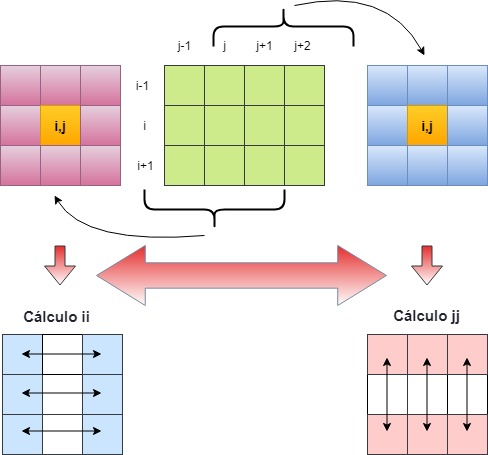
\includegraphics[scale=0.60]{img/bordes1.jpg}
	\caption{Representación del procesamiento de 2 pixeles por ciclo}
	\label{bordes1}
  \end{center}
\end{figure}

{\centering\textbf{Preparación cálculo ii y jj:}}

Se realizará una copia de cada registro \textbf{XMM} que contiene los pixeles de las 3 filas consecutivas, para poder extender los componentes B,G,R,A de cada pixel a tamaño word. \\
Y se procederá a copiar los registros necesarios con estos nuevos componentes de tamaño word para el cálculo de jj y no tener que volver a leerlos de memoria. \\


{\centering\textbf{Cálculo ii:}}

Ahora con los componentes de tamaño word se procede a sacar las diferencias de cada fila respecto a las columnas [ii][j-1] y [ii][j+1] con las instrucciones \textbf{PSUBW} y \textbf{PABSW}. \\
Para luego hacer la sumatoria de estas diferencias con \textbf{PADDW}. \\

{\centering\textbf{Cálculo jj:}}

Se procede a sacar las diferencias de cada columna de las filas [i-1][jj] e [i+1][jj] con las instrucciones \textbf{PSUBW} y \textbf{PABSW}.
Ahora en este caso, en un registro \textbf{XMM} se tendrán las siguientes diferencias  abs([i-1][j-1]-[i+1][j-1]) y abs([i-1][j]-[i+1][j]), y en otro  abs([i-1][j+1]-[i+1][j+1]) y abs([i-1][j+2]-[i+1][j+2]), por lo que hay datos demás para los pixeles que se van a escribir, es por eso que se deben separar datos y no falten ni sobren valores. \\ Para eso se hace una copia y shifts para obtener los resultados deseados.

Se prosigue con la suma de los valores finales de ii y jj, para luego unirlos mediante la instrucción \textbf{POR} con los valores de [\textbf{transparencia}]. Finalmente se convierten los datos a byte sin signo con saturación, se cargan en la imagen \textbf{dst} y se procede al siguiente ciclo o su salida.

